%%%%%%%%%%%%%%%%%%%%%%%%%%%%%%%%%%%%%%%%%
% Structured General Purpose Assignment
% LaTeX Template
%
% This template has been downloaded from:
% http://www.latextemplates.com
%
% Original author:
% Ted Pavlic (http://www.tedpavlic.com)
%
% Note:
% The \lipsum[#] commands throughout this template generate dummy text
% to fill the template out. These commands should all be removed when 
% writing assignment content.
%
%%%%%%%%%%%%%%%%%%%%%%%%%%%%%%%%%%%%%%%%%

%----------------------------------------------------------------------------------------
%	PACKAGES AND OTHER DOCUMENT CONFIGURATIONS
%----------------------------------------------------------------------------------------

\documentclass{article}

\usepackage{fancyhdr} % Required for custom headers
\usepackage{lastpage} % Required to determine the last page for the footer
\usepackage{extramarks} % Required for headers and footers
\usepackage{graphicx} % Required to insert images
\usepackage{lipsum} % Used for inserting dummy 'Lorem ipsum' text into the template
\usepackage{enumerate}
\usepackage{booktabs}
\usepackage{amsmath}

% Margins
\topmargin=-0.45in
\evensidemargin=0in
\oddsidemargin=0in
\textwidth=6.5in
\textheight=9.0in
\headsep=0.25in 

\linespread{1.5} % Line spacing

% Set up the header and footer
\pagestyle{fancy}
\lhead{\hmwkAuthorName} % Top left header
\chead{\hmwkClass\ (\hmwkTitle)} % Top center header
%%\rhead{\firstxmark} 
\rhead{} % Top right header
\lfoot{\lastxmark} % Bottom left footer
\cfoot{} % Bottom center footer
\rfoot{Page\ \thepage\ of\ \pageref{LastPage}} % Bottom right footer
\renewcommand\headrulewidth{0.4pt} % Size of the header rule
\renewcommand\footrulewidth{0.4pt} % Size of the footer rule

\setlength\parindent{0pt} % Removes all indentation from paragraphs

%----------------------------------------------------------------------------------------
%	DOCUMENT STRUCTURE COMMANDS
%	Skip this unless you know what you're doing
%----------------------------------------------------------------------------------------

% Header and footer for when a page split occurs within a problem environment
\newcommand{\enterProblemHeader}[1]{
\nobreak\extramarks{#1}{#1 continued on next page\ldots}\nobreak
\nobreak\extramarks{#1 (continued)}{#1 continued on next page\ldots}\nobreak
}

% Header and footer for when a page split occurs between problem environments
\newcommand{\exitProblemHeader}[1]{
\nobreak\extramarks{#1 (continued)}{#1 continued on next page\ldots}\nobreak
\nobreak\extramarks{#1}{}\nobreak
}

\setcounter{secnumdepth}{0} % Removes default section numbers
\newcounter{homeworkProblemCounter} % Creates a counter to keep track of the number of problems

\newcommand{\homeworkProblemName}{}
\newenvironment{homeworkProblem}[1][Problem \arabic{homeworkProblemCounter}]{ % Makes a new environment called homeworkProblem which takes 1 argument (custom name) but the default is "Problem #"
\stepcounter{homeworkProblemCounter} % Increase counter for number of problems
\renewcommand{\homeworkProblemName}{#1} % Assign \homeworkProblemName the name of the problem
\section{\homeworkProblemName} % Make a section in the document with the custom problem count
\enterProblemHeader{\homeworkProblemName} % Header and footer within the environment
}{
\exitProblemHeader{\homeworkProblemName} % Header and footer after the environment
}

\newcommand{\problemAnswer}[1]{ % Defines the problem answer command with the content as the only argument
\noindent\framebox[\columnwidth][c]{\begin{minipage}{0.98\columnwidth}#1\end{minipage}} % Makes the box around the problem answer and puts the content inside
}

\newcommand{\homeworkSectionName}{}
\newenvironment{homeworkSection}[1]{ % New environment for sections within homework problems, takes 1 argument - the name of the section
\renewcommand{\homeworkSectionName}{#1} % Assign \homeworkSectionName to the name of the section from the environment argument
\subsection{\homeworkSectionName} % Make a subsection with the custom name of the subsection
\enterProblemHeader{\homeworkProblemName\ [\homeworkSectionName]} % Header and footer within the environment
}{
\enterProblemHeader{\homeworkProblemName} % Header and footer after the environment
}
   
%----------------------------------------------------------------------------------------
%	NAME AND CLASS SECTION
%----------------------------------------------------------------------------------------

\newcommand{\hmwkTitle}{Homework\ \#3} % Assignment title
\newcommand{\hmwkDueDate}{Tuessday,\ February\ 13,\ 2018} % Due date
\newcommand{\hmwkClass}{FIN\ 513} % Course/class
\newcommand{\hmwkClassTime}{9:30am} % Class/lecture time
\newcommand{\hmwkAuthorName}{Wanbae Park} % Your name

%----------------------------------------------------------------------------------------
%	TITLE PAGE
%----------------------------------------------------------------------------------------

\title{
\vspace{2in}
\textmd{\textbf{\hmwkClass:\ \hmwkTitle}}\\
\normalsize\vspace{0.1in}\small{Due\ on\ \hmwkDueDate}\\
\vspace{3in}
}

\author{\textbf{\hmwkAuthorName}}
\date{} % Insert date here if you want it to appear below your name

%----------------------------------------------------------------------------------------

\begin{document}

\maketitle

%----------------------------------------------------------------------------------------
%	TABLE OF CONTENTS
%----------------------------------------------------------------------------------------

%\setcounter{tocdepth}{1} % Uncomment this line if you don't want subsections listed in the ToC

%%\newpage
%%\tableofcontents
\newpage

%----------------------------------------------------------------------------------------
%	PROBLEM 1
%----------------------------------------------------------------------------------------

% To have just one problem per page, simply put a \clearpage after each problem

\begin{homeworkProblem}
	The put-call parity of American options on a currency is $e^{-r_f(T - t)}S - K \leq C - P \leq S - e^{-r_d(T-t)}K$ or $B^f S - K \leq C - P \leq S - B^dK$, where $S$ and $K$ denotes spot exchange rate and strike price as usual, $r_d$ and $r_f$ denotes domestic risk-free rate and foreign risk-free rate, respectively.	\\
	\\
	\textit{(Proof)} Suppose not.
	\begin{enumerate}
		\item Suppose $C - P > S - e^{-r_d(T - t)}K$. Then an arbitrage opportunity exists by constructing the following portfolio.
		\begin{enumerate}
			\item Buy a put option and a unit of foreign currency.
			\item Write a call option and borrow $e^{-r_d(T - t)}K$ amount of domestic currency on risk-free rate.
		\end{enumerate}
		All possible situations can be separated by two cases: early exercise of written option occurs and no early exercise of written option. Assuming that early exercise occurs at $t^* < T$, payoff of the portfolio is as follows.
		\begin{enumerate}[\text{\textit{Case}} 1.]
		\item Early exercise at $t^* < T$ occurs.
			\begin{enumerate}[(a)]
				\item $e^{r_f(t^* - t)}S_{t^*}$
				\item $-(S_{t^*} - K)  - e^{-r_d(T - t^*)}K$
			\end{enumerate}
			The sum of payoff from two strategies is $(e^{r_f(t^* - t)} - 1)S_{t^*} + (1 - e^{-r_d(T - t^*)})K$, which is positive.
		\item No early exercise.
			\begin{enumerate}
				\item $S_T > K$
				\begin{enumerate}[(a)]
					\item $0 + e^{r_f(T - t)}S_T$
					\item $-(S_T - K) - K$
				\end{enumerate}
				\item $S_T \leq K$
				\begin{enumerate}[(a)]
					\item $(K - S_T) + e^{r_f(T - t)}S_T$
					\item $0 - K$
				\end{enumerate}
			\end{enumerate}
			In this case, the portfolio also has a positive payoff regardless of spot exchange rate at maturity.
		\end{enumerate}
		Since the portfolio has a positive payoff at all possible situations, there must be a cost for implementing the strategies if there is no arbitrage opportunity. However, by the assumption, the initial cost for constructing portfolio is negative, so a contradiction occurs. Therefore, $C - P \leq S - e^{-r_d(T - t)}K$ must hold.
%----------------------------------------------------------------------------------------
		\item Suppose $C - P < e^{-r_f(T - t)}S - K$. Then there is also an arbitrage opportunity exists considering the following portfolio.
		\begin{enumerate}
			\item Buy a call option and invest K amount of domestic currencies on domestic risk-free rate.
			\item Write a put option and sell short a foreign risk-free zero coupon bond.
		\end{enumerate}
		By using similar procedure above, existence of arbitrage can be derived.
		\begin{enumerate}[\text{\textit{Case}} 1.]
			\item Early exercise at $t^* < T$ occurs.
			\begin{enumerate}[(a)]
				\item $e^{rt^*}K$
				\item $-(K - S_{t^*}) - e^{-r_f(T - t^*)}S_{t^*}$
			\end{enumerate}
			In this case, the sum of payoff from two strategies above is $S_{t^*}(1 - e^{-r_f(T - t^*)}) - (e^{rt^*} - 1)K$, which is positive.
			\item No early exercise.
			\begin{enumerate}
				\item $S_T > K$
				\begin{enumerate}[(a)]
					\item $(S_T - K) + e^{r(T - t)}K$
					\item $0 - S_T$
				\end{enumerate}
				\item $S_T \leq K$
				\begin{enumerate}[(a)]
					\item $0 + e^{r(T - t)}K$
					\item $-(K - S_T) - S_T$
				\end{enumerate}
			\end{enumerate}
			At the maturity, the portfolio has a positive value regardless of spot exchange rate at $T$.
		\end{enumerate}
		Since the portfolio has a positive payoff at all possible situations, there is an arbitrage opportunity since we assumed that there is a negative initial cost for constructing this portfolio. Therefore, $C - P \geq e^{-r_f(T - t)}S - K$ must hold.
	\end{enumerate}
	Combining all results above, the put-call parity mentioned above must hold. Otherwise, there would be an arbitrage opportunity.
\end{homeworkProblem}
%----------------------------------------------------------------------------------------
%	PROBLEM 2
%----------------------------------------------------------------------------------------
\begin{homeworkProblem}
\begin{enumerate}[(a)]
	\item %%(a)
	\textbf{False.} Even if $c(K, T) > S_t$, in order to lock arbitrage profit in, it needs to trade underlying asset. However, in this case, underlying asset is not tradable, constructing arbitrage portfolio is impossible.
%----------------------------------------------------------------------------------------
	\item %%(b)
	\textbf{True.} Suppose $p(K, T) > B_{t, T} \cdot  K$. Then by selling short a put option with strike price $K$ and maturity $T$, and buying a zero coupon bond with face value $K$ and maturity $T$. Note that there is a negative initial cost. If a spot price is larger than strike price at maturity, the payoff of portfolio would be equal to $K > 0$. Otherwise, the payoff would be equal to $-(K - S_T) + K = S_T$, which is also positive. Therefore, even if underlying asset is not tradable, by making a transaction of options and bonds, it is possible to make arbitrage profit.
%----------------------------------------------------------------------------------------
	\item %%(c)
	\textbf{False.} Suppose $c(K, T_1) > c(K, T_2)$. Based on the principle of `buy low, sell high', construct a portfolio by selling short $c(K, T_1)$ and buying $c(T, K_2)$. If spot price at $T_1$ is less than $K$, net profit would be positive since the written option would not be exercised. In contrast, if spot price at $T_1$ is greater than $K$, a negative payoff $K - S_T$ would be generated, and to make an arbitrage profit, it needs to deal with this payoff. Since the portfolio consists of a call option maturing at $T_2$, selling short an underlying asset and investing $K$ amount of dollars on risk free rate would make an arbitrage profit. However, since the underlying asset is non-tradable, implementing this strategy is impossible. It means that even if $c(K, T_1) > c(K, T_2)$, locking in an arbitrage profit is impossible.
%----------------------------------------------------------------------------------------
	\item %%(d)
	\textbf{False.} The put-call parity assumes that tradable underlying asset. Since it is impossible to trade the underlying asset, put call parity does not hold.
%----------------------------------------------------------------------------------------
	\item %%(e)
	\textbf{True.} Regardless of spot value, it is possible to make positive payoff by selling short two $c(K_1, T)$, and buying a $c(K_0, T)$ and $c(K_2, T)$. Since the strategy does not contain any underlying asset, if $c(K_0, T) - 2(K_1, T) + c(K_2, T) \leq 0$, it is possible to make an arbitrage profit without trading underlying asset. Therefore, $c(K_0, T) - 2(K_1, T) + c(K_2, T)$ should be positive.
%----------------------------------------------------------------------------------------
	\item %%(f)
	\textbf{False.} If $c(K_2, T) \geq c(K_1, T)$, then arbitrage is possible. Construct a portfolio by selling short a $c(K_2, T)$ and buying a $c(K_1, T)$. Then it is possible to make an arbitrage profit. Table \ref{tab:prob2(f)-payoff} shows details about arbitrage profit.
%----------------------------------------------------------------------------------------
	%% PAYOFF TABLE
	\begin{table}[h]
	\centering
	\label{my-label}
	\begin{tabular}{@{}cccc@{}}
	\toprule
                    & $S_T < K_1$ & $K_1 \leq S_T < K_2$ & $K_2 \leq S_T$ \\ \midrule
	\textit{Long call}  & 0           & $S_T - K_1$          & $S_T - K_1$    \\
	\textit{Short call} & 0           & 0                    & $-(S_T - K_2)$ \\	\midrule
	\textit{Sum}        & 0           & $S_T - K_1$          & $K_2 - K_1$    \\ \bottomrule
	\end{tabular}
	\caption{Payoff of portfoliio}	\label{tab:prob2(f)-payoff}
	\end{table}
%----------------------------------------------------------------------------------------
	\item %%(g)
	\textbf{False.} Proving $p(K, T) \geq \text{max}(B_{t, T} \cdot K - S_t, 0)$ is equivalent to proving $p(K, T) \geq B_{t, T} \cdot K - S_t$ since option price is always greater than zero. Nevertheless, even though $p(K, T) \leq B_{t, T} \cdot K - S_t$, it is impossible to make an arbitrage profit. Since the formula contains $S_t$, it is inevitable to transact underlying asset to make an arbitrage profit. Therefore, since the underlying asset is non-tradable, making an arbitrage profit is impossible in this case.
%----------------------------------------------------------------------------------------
	\item %%(h)
	\textbf{True.} Suppose $C(K, T) < c(K, T)$. Then by selling short European option and buying equal amount of American option, it is possible to make an arbitrage profit. It is because it is always possible to net European payoff out by exercising American option at maturity. Therefore, $C(K, T) \geq c(K, T)$ must hold.
\end{enumerate}
\end{homeworkProblem}
%----------------------------------------------------------------------------------------
%	PROBLEM 3
%----------------------------------------------------------------------------------------
\begin{homeworkProblem}
\begin{enumerate}[(a)]
	\item Figure \ref{fig:prob3-function} represents plots of function $f$, $g$, $h$ over the range -1 to 2.
	\begin{figure}[h]
		\begin{center}
		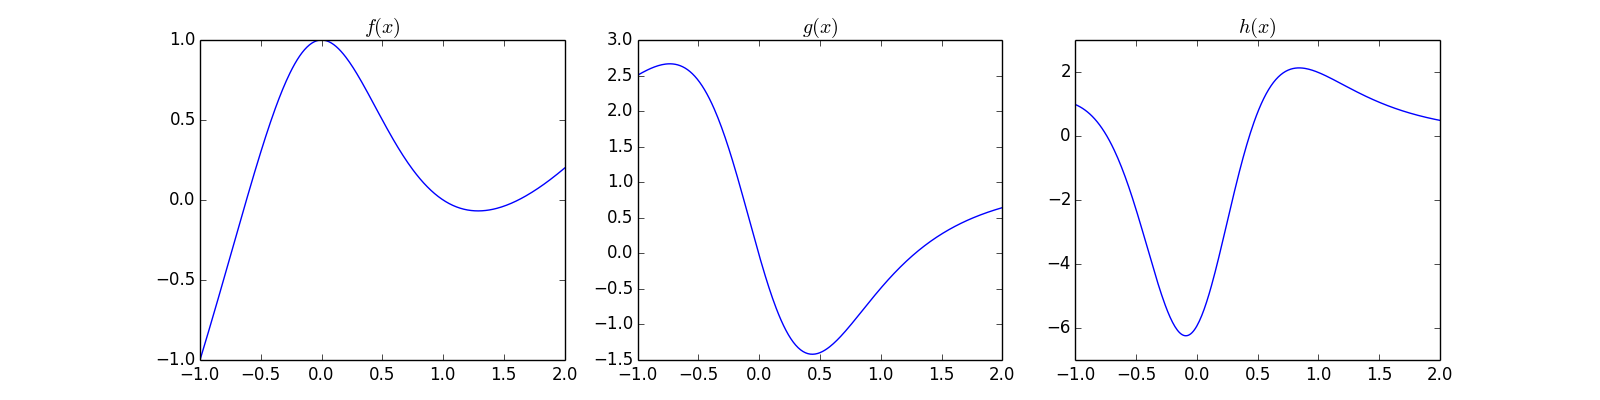
\includegraphics[scale = 0.4]{function.png}
		\caption{$f(x)$, $g(x)$, $h(x)$ (from left to right)}
		\label{fig:prob3-function}
		\end{center}
	\end{figure}
	\item
	From the figure \ref{fig:prob3-function}, it seems that from $x = 0.5$(approximately) the function $f$ is convex since its slope starts increase at this point. Actually, using some calculus, since $h(x) = -\frac{2(x^3 - 9x^2 - 3x + 3)}{(x^2 + 1)^3}$, $f(x)$ is convex from $x = 0.4422$.
	\item
	It appears that from $x = -0.1$ to 0.8(approximately) the function looks convex. It is because function $h(x)$ starts to increase at -0.1 and stops increasing at 0.8.
	\item
	Visually, it seems that from $x = -0.5$ to 0.4 $h(x)$ looks convex.
\end{enumerate}
\end{homeworkProblem}
%----------------------------------------------------------------------------------------
%	PROBLEM 4
%----------------------------------------------------------------------------------------
\begin{homeworkProblem}
\begin{enumerate}[(a)]
	\item
	There is an arbitrage opportunity. Since the probabilities mentioned are exact, there is just two possibilities that stock price moves up to \$120 or down to \$90, so if someone sell short a call option with strike price 120, then there would be an arbitrage because the price of call option is positive and there is no amount pay at maturity with certainty. 
	\item
	As long as the statistical probabilities are true, using the idea of binomial tree, option price should be equal to followings.
	\begin{equation*}
	\begin{aligned}
		c(100) 	&= e^{-0.06 \times \frac{1}{12}}(0.4 \times 20 + 0.6 \times 0)	\\
				&= 7.96	\\
		c(110) 	&= e^{-0.06 \times \frac{1}{12}}(0.4 \times 10 + 0.6 \times 0)	\\
				&= 3.9	\\
		c(120) 	&= e^{-0.06 \times \frac{1}{12}}(0.4 \times 0 + 0.6 \times 0)	\\	
				&= 0	
	\end{aligned}
	\end{equation*}
	However, it is totally different from the price of options traded in the market. There are two possibilities that makes deviation between theoretical prices and market prices. First, there would be differences between statistical probabilities and market-implied probabilities. One main reason why $c(100)$ and $c(110)$ using statistical probabilities is higher than market prices is because relatively higher (statistical) probability is allocated to the state that stock prices moves up to 120. In other words, if a probability less than 0.4 is allocated to the state in which stock price goes up to 120, $c(100)$ and $c(110)$ would be closer to the market price. Second, there would be more states rather than two states. Regarding the statistical probabilities, there are just two states, and under those states $c(120)$ is always equal to zero whatever probabilities are allocated to. It means that market prices of option imply that there are more states than statistical view, especially states that stocks price will be larger than 120. Summing up, statistical probabilities assumes more simple states than market implied view, and allocate more probabilities to states that stock prices are larger than 100.
\end{enumerate}
\end{homeworkProblem}
\end{document}
